\documentclass[11pt,a4paper]{jsarticle}
%
\usepackage{amsmath,amssymb}
\usepackage{bm}
\usepackage[dvipdfmx]{graphicx}
\usepackage[dvipdfmx]{color}
\usepackage{ascmac}
\usepackage{listings}
%
\setlength{\textwidth}{\fullwidth}
\setlength{\textheight}{40\baselineskip}
\addtolength{\textheight}{\topskip}
\setlength{\voffset}{-0.2in}
\setlength{\topmargin}{0pt}
\setlength{\headheight}{0pt}
\setlength{\headsep}{0pt}
%
\newcommand{\divergence}{\mathrm{div}\,}  %ダイバージェンス
\newcommand{\grad}{\mathrm{grad}\,}  %グラディエント
\newcommand{\rot}{\mathrm{rot}\,}  %ローテーション
%
\title{レポート課題2}
\author{05-191009 奥村真司}
\date{}
\begin{document}
\maketitle
%
%
\section*{問1}
\subsection*{動作例}
\begin{lstlisting}[basicstyle=\ttfamily\footnotesize, frame=single]
# let five = i2n 5;;
val five : nat = S (S (S (S (S Z))))
# let three = i2n 3;;
val three : nat = S (S (S Z))
# add five three;;
- : nat = S (S (S (S (S (S (S (S Z)))))))
# sub five three;;
- : nat = S (S Z)
# mul five three;;
- : nat = S (S (S (S (S (S (S (S (S (S (S (S (S (S (S Z))))))))))))))
# n2i (pow five three);;
- : int = 125
# n2i (mul five three);;
- : int = 15
\end{lstlisting}
\subsection*{考察}
まずnat型はパターンマッチによってZかSの判定をし、Sならば1引いたものがとれる(すなわち$\texttt{|S p -> ...}$)ことに注意する。add,sub,mul,powは第2引数をパターンマッチで場合分けし、一つ小さい場合に帰着して再帰した。他も同様にZになるまで一つずつ小さいものに帰着して再帰した。
\section*{問2}
\subsection*{動作例}
\begin{lstlisting}[basicstyle=\ttfamily\footnotesize, frame=single]
# let t = Node(1,Node(2,Node(3,Leaf,Leaf),Node(4,Leaf,Leaf)),
Node(5,Node(6,Leaf,Leaf),Node(7,Leaf,Leaf)));;
val t : int tree =
  Node (1, Node (2, Node (3, Leaf, Leaf), Node (4, Leaf, Leaf)),
   Node (5, Node (6, Leaf, Leaf), Node (7, Leaf, Leaf)))
# dfs_pre t;;
- : int list = [1; 2; 3; 4; 5; 6; 7]
# dfs_in t;;
- : int list = [3; 2; 4; 1; 6; 5; 7]
# dfs_pos t;;
- : int list = [3; 4; 2; 6; 7; 5; 1]
\end{lstlisting}
\subsection*{考察}
今いる頂点をn,左の部分木をl,右の部分木をrとする。行きがけ順はまずnをマークしてから次にlの中を行きがけ順でマークして、次にrの中を行きがけ順でマークする順であり、通りがけ順はl,n,rの順、帰りがけ順はl,r,nの順である。二分木の型の定義よりこれらn,l,rはパターンマッチで簡単に得られるので各々の順の決まりをそのまま再帰で実装してやるとそれぞれの順で並べたリストが得られる。
\section*{問3}
\subsection*{動作例}
\begin{lstlisting}[basicstyle=\ttfamily\footnotesize, frame=single]
# let t = Node(1,Node(2,Node(3,Leaf,Leaf),Node(4,Leaf,Leaf)),
Node(5,Node(6,Leaf,Leaf),Node(7,Leaf,Leaf)));;
val t : int tree =
  Node (1, Node (2, Node (3, Leaf, Leaf), Node (4, Leaf, Leaf)),
   Node (5, Node (6, Leaf, Leaf), Node (7, Leaf, Leaf)))
# bfs t;;
- : int list = [1; 2; 5; 3; 4; 6; 7]
\end{lstlisting}
\subsection*{考察}
幅優先探索の順に出力したいのでqueueがあれば良い。listを後ろへの挿入に時間のかかるqueueと思って、BFSをしてリストを作った。現在のqueueと作成途中のリストを引数にとって末尾再帰で実装した。
\section*{問4}
\subsection*{定義}
\begin{lstlisting}[basicstyle=\ttfamily\footnotesize, frame=single]
type expr =
| EConstInt of int
| EAdd of expr * expr
| ESub of expr * expr
| EMul of expr * expr
| EConstBool of bool
| Eequal of expr * expr
| Elt of expr * expr
| Eif of expr * expr * expr;;
type value = VInt of int | VBool of bool;;
\end{lstlisting}
\subsection*{考察}
BNFの通り定義するだけ。
\section*{問5}
\subsection*{動作例}
\begin{lstlisting}[basicstyle=\ttfamily\footnotesize, frame=single]
# eval (EAdd (EConstInt 5,(EMul (EConstInt 2,EConstInt 3))));;
- : value = VInt 11
# eval (EAdd (EConstInt 5,(EMul (EConstInt 2,EConstBool false))));;
Exception: Eval_error.
# eval (Eif ((Eequal (EConstInt 5,EAdd (EConstInt 2,EConstInt 3))),
EConstInt 4,EConstBool true));;
- : value = VInt 4
# eval (Eif ((Eequal (EConstInt 5,EAdd (EConstInt 2,EConstInt 2))),
EConstInt 4,EConstBool true));;
- : value = VBool true
# eval(EDiv (EConstInt 5,ESub (EConstInt 3,EConstInt 1)));;
- : value = VInt 2
# eval(EDiv (EConstInt 5,ESub (EConstInt 3,EConstInt 2)));;
- : value = VInt 5
# eval(EDiv (EConstInt 5,ESub (EConstInt 3,EConstInt 3)));;
Exception: Eval_error.
# eval (Eif ((Eequal (EConstInt 5,EAdd (EConstInt 2,EConstInt 3))),
  EConstInt 4,EAdd (EConstInt 3,EConstBool true)));;
- : value = VInt 4
\end{lstlisting}
\subsection*{考察}
基本的にはパターンマッチで型がおかしくないかを検査する。EAdd等の四則演算では両引数の評価結果がVIntかどうかをチェックしてから演算をする。
Eltはbool同士の演算もできる仕様とした。(trueのほうがfalseより大きい)\par
また、Eifにおいては第一引数の評価結果によって一方のみが評価されるようにしたので評価されない方の式が不正(boolとintの足し算など)でも、エラーを返さないという仕様にした。(上の動作例で最後の例)
\section*{発展1}
\subsection*{動作例}
\begin{lstlisting}[basicstyle=\ttfamily\footnotesize, frame=single]
# let sum_to_sub = fun f n -> if n=0 then 0 else n + f (n-1);;
val sum_to_sub : (int -> int) -> int -> int = <fun>
# let sum_to = fun x -> fix sum_to_sub x;;
val sum_to : int -> int = <fun>
# sum_to 5;;
- : int = 15
# sum_to 10;;
- : int = 55
\end{lstlisting}
\subsection*{考察}
$\texttt{let rec}$を用いずに再帰関数を定義するために問2の二分木などで扱った再帰的な型の定義に着目し、それを利用した。advanced1.ml内で定義されている$\texttt{recfunc}$型は、それ自身を引数として[何か]を返す関数である。この定義によってrecfunc型の関数は自分自身を引数としてとることができる。$\texttt{rec\_call}$でやっていることがこれである。\par
今回最終的にfixを作りたいので[何か]はfixと同じ型の関数とした。$\texttt{fix\_rec}$は、recfunc型で$\texttt{rec\_call\ fix\_rec}$がfixと同等の関数を返すようなものである。定義を見るとわかるように、$\texttt{fix\_rec}$は自分自身(self)を引数にとると、返すときに自分に自分を食わせる($\texttt{rec\_call\ self}$)ようになっておりこれが再帰的に起こることで、fixの再帰が実現されている。fixは第1回でやったとおりfix f x = f (fix f) xをみたすものだったのでこれと合致するように$\texttt{fix\_rec}$を定義した。
\section*{発展2}
\subsection*{動作例}
\begin{lstlisting}[basicstyle=\ttfamily\footnotesize, frame=single]
# #use "advanced2.ml";;
type false_t = { t : 'a. 'a; }
type 'a not_t = 'a -> false_t
type ('a, 'b) and_t = 'a * 'b
type ('a, 'b) or_t = L of 'a | R of 'b
val top : 'a -> 'a = <fun>
val orE : ('a, 'b) or_t -> ('a -> 'c) -> ('b -> 'c) -> 'c = <fun>
val func1 : ('a -> 'b) -> ('b -> 'c) -> 'a -> 'c = <fun>
val func2 : ('a, ('b, 'c) and_t) or_t -> (('a, 'b) or_t, ('a, 'c) or_t) and_t =
  <fun>
val func3 : (('a, 'b) or_t, ('a, 'c) or_t) and_t -> ('a, ('b, 'c) and_t) or_t =
  <fun>
val callcc : (('a -> false_t) -> 'a) -> 'a = <fun>
val func4 : ('a -> 'c) -> ('a not_t -> 'c) -> 'c = <fun>
val func6 : (('a -> 'b) -> 'a) -> 'a = <fun>
\end{lstlisting}
\subsection*{考察}
カリーハワード対応より直観主義論理で示すことができる命題に対応する型ならば再帰、副作用なしで定義可能で、実際1,2,3は定義できた。(単純なので証明図は省略する) \par
4は排中律だが、直観主義論理では示せないので再帰、副作用なしでは定義できない。5も直観主義論理において偽の命題なので定義できない。6のPeirce則も同様に定義できない。\par
次にcallccを許す場合を考える。callccを許すと古典論理で証明可能な命題に対応する型のものなら定義可能になる。よって4,6が定義できる。5は古典論理においても偽の命題なので定義できない。callccの型はスライドにあるとおり$\texttt{(not\ A\ ->\ A)\ ->\ A}$である。直観主義論理の推論規則にcallccを公理として加えた体系での4,6の証明図を以下に載せる。(打ち込むのが面倒で手書きです、すみません)
\begin{figure*}
  \begin{center}
    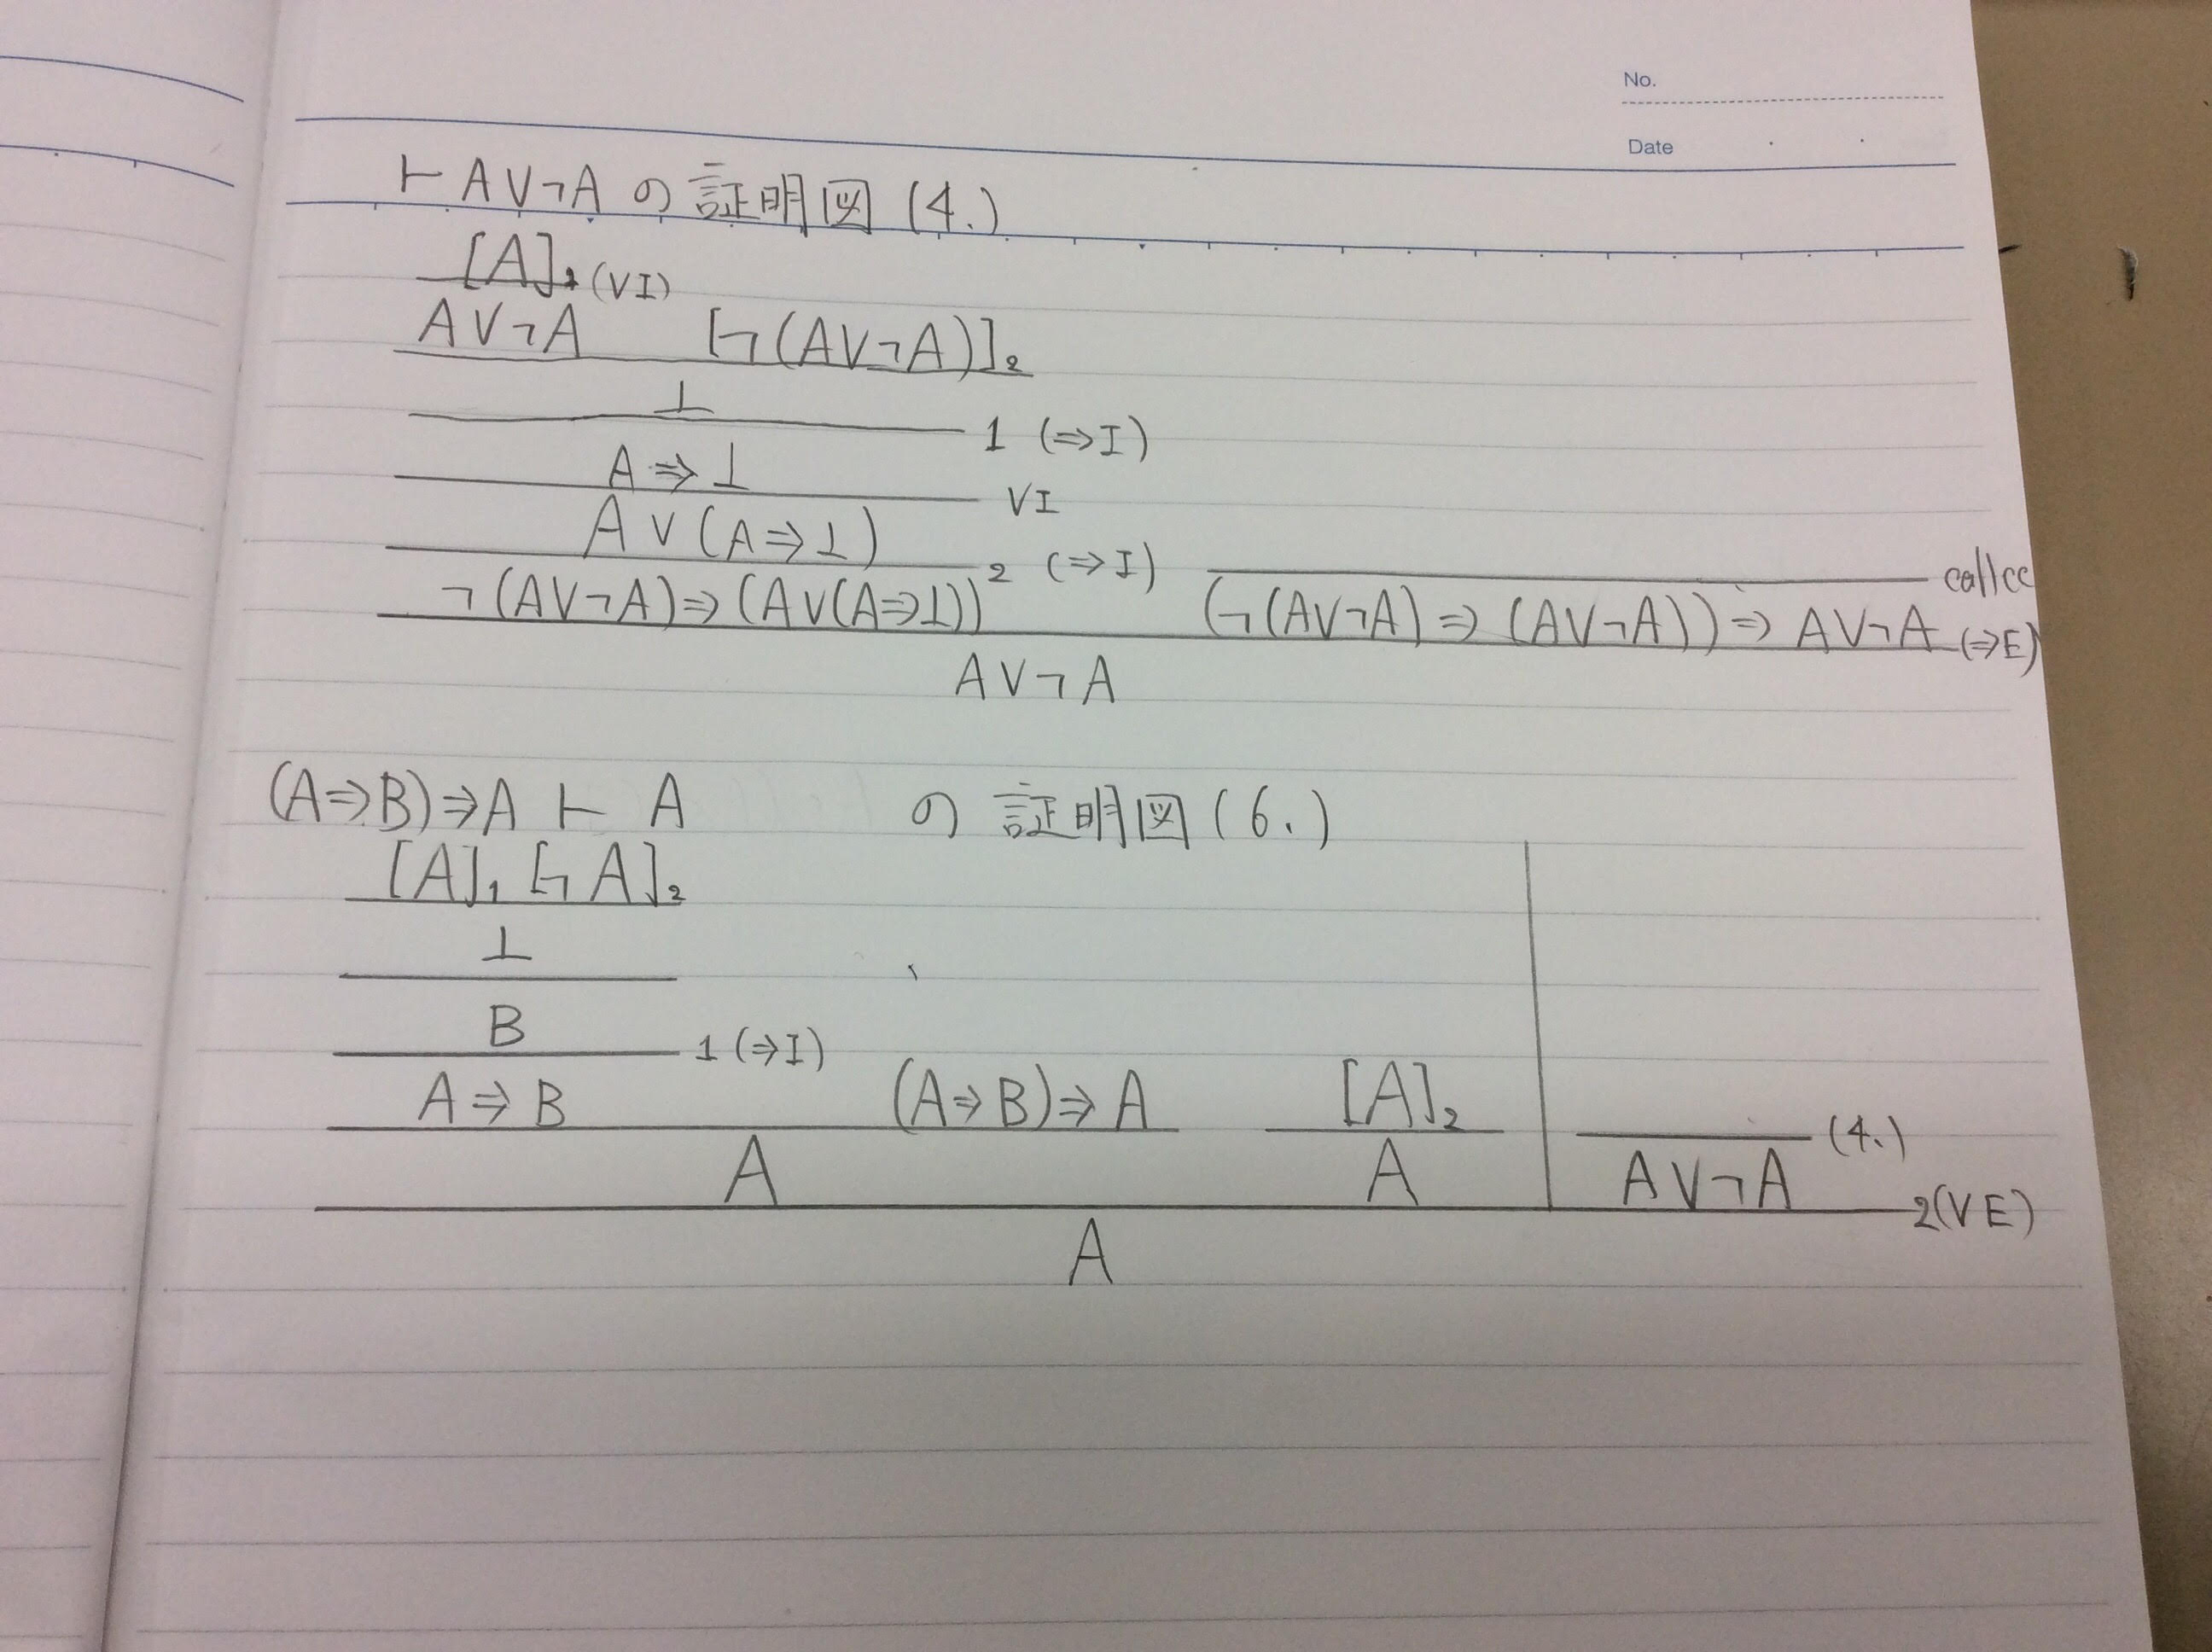
\includegraphics[width=15cm]{proof.jpg}
  \end{center}
\end{figure*}
4の証明図の最後のステップでは$\texttt{not\ A}$が$\texttt{A\ -> bottom}$であることを用いています。
この証明図の流れに沿って順に組み立てていくことでadvanced2.ml内のfunc4,func6が定義できた。今回callccを型だけ合うように定義して代用しているため4でスライドの上の式を作ろうとするとこれは値なので評価が始まって代用しているcallccの実装のせいで無限ループしてしまうため下の式の型の関数を定義した。
\end{document}
